% Set the author and title of the compiled pdf
\hypersetup{
  pdftitle = {\Title},
  pdfauthor = {\Author}
}

\section{Algorithmic Wisdom}

{\hspace{2.2em} \small Lectures 2 \& 3}

The first two lectures of the course describe different types of algorithms,
what is computable, where to optimise algorithms, asymptotics and heuristics.

\subsection{Different types of algorithms}

There are three types of algorithms that are mentioned:

\marginpar{You should know all of this from \texttt{COMP26120}.}

\begin{description}
  \item \textbf{Divide and conquer}\\
  These algorithms continually break a problem down into smaller parts, which
  are easier to solve, until eventually, the problems are trivial and easily
  solved. This is often used when the data you're operating on is in a
  recursive datastructure such as a tree. If you're writing an algorithm to
  find how many nodes there are in a tree, then you could use divide and
  conquer:

  \begin{lstlisting}[language=java]
    int countTreeSize(tree) {
    int size = 1;
    if (tree.left) size += countTreeSize(tree.left);
    if (tree.right) size += countTreeSize(tree.right);
    return size;
    }
  \end{lstlisting}

  As you can see from the example, divide and conquer algorithms are usually
  recursive.

  The divide and conquer technique can be applied to graphs, but in order to
  do this, you must keep track of which nodes you've visited with a flag on
  each node. If we wanted to count the nodes in a graph, we could do:

  \begin{lstlisting}[language=java]
    int countGraphSize(graph) {
    if (graph.visited) return 0;
    graph.visited = true;
    int size = 1;
    for (child in graph) {
      size += countGraphSize(child);
    }
    return size;
    }
  \end{lstlisting}

  \item \textbf{Mutual Recursion}\\
  Mutual recursion describes an algorithm that operates on data where one type
  of data can reference another, and the other can reference it. The example
  given is that of statements and expressions in programming languages;
  statements contain expressions, and expressions can also contain statements.
  Parsing such a structure might involve two algorithms that recurse on each
  other!

  \item \textbf{Dynamic Programming}\\
  Dynamic programming exploits the fact that when some problems are broken
  down into smaller sub-problems, some of the sub-problems are identical.
  Dynamic programming algorithms start from the very smallest sub-problems and
  build up to the final solution, and usually cache results to sub-problems in
  a table so that work is not done twice.

\end{description}

\subsection{Computability}
% TODO: Combine this with a later topic?

There are many different definitions of computability, including
\href{https://en.wikipedia.org/wiki/Lambda_calculus}{lambda calculus},
\href{https://en.wikipedia.org/wiki/Turing_machine}{Turing machines},
\href{https://en.wikipedia.org/wiki/Rewriting}{rewriting rules},
\href{https://en.wikipedia.org/wiki/Random-access_machine}{random access
machines} and (many) more. The idea that relates all of these things, is that
they all have the same capabilities. That is to say that if you can compute
something using one of these ideas, then you can also compute it on all the
others too.

There are also a class of `alternate' computing mechanisms, such as quantum
computers and neural computers. These ideas have the potential to compute things
that a Turing machine (or its equivalents cannot), but they are significantly
harder to build, and functional implementations do not exist yet.

\subsection{Asymptotics and optimisation}

When you have to get a computer to perform a task, implementing a simple
algorithm first is a good idea, since you will at least have something to
demonstrate to people, and you will gain a good understanding of the problem at
hand. However, simple algorithms are often slow; how should we evolve our
implementation to be as fast as we need it to be?

Profiling can tell you where your code is spending most of its time. Sometimes
your algorithm will be really fast, and the processor will spend most of its
time waiting for IO to give it more data; this is often the case with GPU
computation.

Assuming you find some CPU bottleneck in your code, before you spend hours
making it faster, consider whether it is worth the effort. If this part takes up
10\% of your runtime, and you make it twice as fast, your program will only run
5\% faster. This is an example of the
\href{https://en.wikipedia.org/wiki/Diminishing_returns}{Law of Diminishing
Returns}.

As well as optimising specific parts of an algorithm, you also should consider
its asymptotic run time. An algorithm that runs in $O(n^2)$ time is probably
going to be better than one that runs in $O(n log(n))$ time. However, this isn't
always the case; some algorithms (often ones with good asymptotic run times)
take a long time to set up, usually when you have to transform the data into
some different datastructure. If you are running your algorithm on a small
amount of data, then an algorithm that you can run on your data \textit{as is}
might outperform a fancier algorithm that you have to invest more overhead in.

\marginpar{Sometimes a good solution is to use different algorithms depending
on the input. If there are only a few cases that produce worst-case performance,
you could even hard-code solutions to those!}

The average case runtime of a algorithm is also important. Haskell uses a type
checker that runs in $O(2^{n^n})$ time in the worst case, but for every program
that isn't made specifically to mess with the compiler, runs in linear time.

\section{Graphs}

A graph is a pair $G = (V,E)$ where $V$ is a finite set, and $E$ is a set of
pairs between items in $V$. Elements in $V$ are \textit{vertices} or
\textit{nodes}, and elements in $E$ are \textit{edges}.

Different mathematicians have different rules about what exactly can go in a
graph. For the purposes of this course, the graphs shown in
Figure~\ref{fig:bad-graphs} aren't allowed.

\begin{figure}[h]
  \centering
  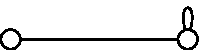
\includegraphics{diagrams/self-loops}\\
  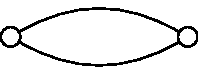
\includegraphics{diagrams/multiple-edges}\\
  
\includegraphics{diagrams/directed-graph}
  \caption{Self loops, duplicate edges and arrows are not allowed.}
  \label{fig:bad-graphs}
\end{figure}

A \textbf{directed graph} is just like a normal graph, except the edges do have
arrows. The only mathematical difference is that the set $E$ is a set of ordered
pairs.

The \textit{degree} of a node in a graph, is the number of edges that are
adjacent to (touching) it. If the graph is directed, then it is the number of
edges originating from the node.

A weighted graph is one where each edge is associated with a value representing
its weight. The length of a path between nodes is simply the sum of the edge
weights connecting the nodes.

\subsection{Connectivity}

A node $a$ is \textbf{reachable} from another node $b$ if there is some sequence
of nodes connected by edges that go from the $a$ to $b$.

A graph where every node is reachable from every other node is
\textbf{connected}. A strongly connected graph is a \textbf{directed graph}
where each node is reachable from each other node.

\begin{figure}[h]
  \centering
  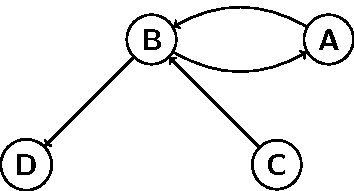
\includegraphics{diagrams/connected-graph}
  \caption{This graph is not strongly connected, but the subgraph with only
  nodes $A$ and $B$ is. If we were to remove the arrows, then the graph would
  be connected.}
  \label{fig:connected-graph}
\end{figure}

\subsection{Representing graphs}

We can store graphs in computer memory in two ways:

\begin{description}
  \item \textbf{Adjacency List}\\
    There are two different kinds of adjacency list, the first is like so:

    \begin{lstlisting}[language=java]
      public class Graph {
        List<Vertex> nodes;
        List<Edge> edges;
      }
      public class Edge { Vertex a, b; }
      public class Vertex { List<Edge> outlist; }
    \end{lstlisting}

    Here, we keep a list of all the nodes, and a list of all the edges. From
    any edge, we can see what nodes it connects, and from any node, we can
    see what edges it connects.

    The other type of adjacency list is a bit simpler, but less efficient in
    some cases:

    \begin{lstlisting}[language=java]
      public class Graph<T> {
        Set<T, List<T>> adjList;
      }
    \end{lstlisting}
  \item \textbf{Adjacency Matrix}\\
    Here, a matrix indicates whether there is an edge between two nodes:

    \begin{center}
      \begin{tabular}{c|c c c c}
          & A & B & C & D\\ \hline
        A & 0 & 1 & 0 & 0\\
        B & 1 & 0 & 0 & 1\\
        C & 0 & 1 & 0 & 0\\
        D & 0 & 0 & 0 & 0\\
      \end{tabular}
    \end{center}

    This adjacency matrix represents the graph in
    Figure~\ref{fig:connected-graph}. You can see that it is fairly wasteful
    in terms of memory $O(|E|* |V|)$, though with bit arrays, it has a very 
    low constant overhead.
\end{description}

\subsection{Graph algorithms}

You will have covered some of the algorithms featuring here in previous courses,
or perhaps seen them in the wild. They are however interesting and useful, so
it's worth a recap even if they're not new! I've ordered these in roughly
increasing order of mental strain.

\subsubsection{Depth first search}

\href{https://en.wikipedia.org/wiki/Depth-first_search}{Depth first search}
(DFS) is an algorithm to find a node in a graph starting from another node. It
works on both directed and undirected graphs, and runs in $O(|V| + |E|)$
(linear) time. The psudo code looks like this:

\begin{lstlisting}[language=java]
  Node dfs(Node haystack, Node needle) {
    Stack<Node> toVisit = new Stack<>();
    Set<Node> visitedNodes = new Set<>();
    toVisit.push(haystack);
    while(!toVisit.isEmpty()) {
      Node node = toVisit.pop();
      if (visitedNodes.contains(node)) continue;
      visitedNodes.add(node);
      if(node.equals(needle)) {
        return needle;
      } else {
        for(Node child : node.children) {
          toVisit.push(child);
        }
      }
    }
    return null;
  }
\end{lstlisting}

A Breadth First Search is the same, except you use a \texttt{Queue} instead of a
\texttt{Stack}.

\marginpar{To see if a graph is connected, do a depth first search as in the
example code, but don't stop when you find a needle, only stop when the
\texttt{toVisit} stack is empty. If \texttt{visitedNodes} contains all of the
nodes in the graph, then the graph is connected.}

Depth first search also lets you find if one node is reachable from another in
linear time, and also if a graph is connected in linear time too, with a few
modifications.

We can also find out if a directed graph is strongly connected in $O(|V| + |E|)$
time using Tarjan's algorithm, which we'll see later.

\subsubsection{Dijkstra's algorithm}

Dijkstra's algorithm finds the undirected shortest path between two nodes in a
graph. Here is the psudo-code:

\begin{lstlisting}[language=java,
                  caption=Dijkstra's algorithm (from Wikipedia),
                  label=lst:dijkstra,
                  captionpos=b]
function Dijkstra(Graph, source):
  create vertex set Q

  for each vertex v in Graph:        // Initialization
    dist[v] = INFINITY               // Unknown distance from source to v
    prev[v] = UNDEFINED              // Previous node in optimal path from source
    add v to Q                       // All nodes initially in Q (unvisited nodes)

  dist[source] = 0                   // Distance from source to source

  while Q is not empty:
    u = vertex in Q with min dist[u] // Source node will be selected first
    remove u from Q 

  for each neighbour v of u:          // where v is still in Q.
    alt = dist[u] + length(u, v)
    if alt < dist[v]:                // A shorter path to v has been found
      dist[v] = alt 
      prev[v] = u 

  return dist[], prev[]
\end{lstlisting}

If we use a Fibonacci heap, for the priority queue, then the runtime of
Dijkstra's algorithm is $O(|E| + |V|log(|V|)$. If we use a normal heap, then the
runtime is $O(|E|log(|V|))$.
